\documentclass [11pt,twoside]{article}
\usepackage[utf8]{inputenc}
\usepackage[T1]{fontenc}

%Page margins, header and footer positions
\usepackage{geometry}
 \geometry{
 a4paper,
 total={210mm,297mm},
 left=25mm,
 right=25mm,
 top=30mm,
 bottom=25mm,
 headsep=7mm}

\interfootnotelinepenalty=10000

%To display filling dots in the TOC for all entries
\usepackage[titles]{tocloft}
\renewcommand{\cftsecleader}{\cftdotfill{\cftdotsep}}

%Define new header and footer style
\usepackage{fancyhdr}

\pagestyle{fancy}
\fancyhf{}
\lhead{\color{Gray}{\small{Travlendar+ project by YOUR NAMES}}}
\lfoot{\textcolor{Gray}{\small{Copyright © 2017, YOUR NAMES – All rights reserved}}}
\rfoot{\textcolor{Gray}{\thepage}}
\renewcommand{\headrulewidth}{0pt}

%PACKAGES
\usepackage{wasysym}
\usepackage{pifont}

\newcommand{\supported}{\ding{52}\xspace}
\newcommand{\unsupported}{\ding{55}\xspace}
\newcommand{\partsupported}{\textcolor{black!40}{\ding{52}}\xspace}
\newcommand{\lowsupported}{\textcolor{black!20}{\ding{52}}\xspace}
\newcommand{\unknowsupported}{\textbf{?}\xspace}

%Font: Times
\usepackage{times}
%Change monospaced font
\renewcommand{\ttdefault}{lmtt}

%tables
\usepackage{tabu}
\usepackage{tabularx}
\usepackage{ltablex}
\usepackage{longtable}
\usepackage{float} % To allow the use of H modifier in long tables

%landscape mode
\usepackage{pdflscape}
\usepackage{rotating}
\usepackage{caption}

%make landscape mode be sensitive to even and odd pages
%start
\def\myrotate{\ifodd\c@page\else-\fi 90}
\makeatletter
\global\let\orig@begin@landscape=\landscape%
\global\let\orig@end@landscape=\endlandscape%
\gdef\@true{1}
\gdef\@false{0}
\gdef\landscape{%
    \global\let\within@landscape=\@true%
    \orig@begin@landscape%
}%
\gdef\endlandscape{%
    \orig@end@landscape%
    \global\let\within@landscape=\@false%
}%
\@ifpackageloaded{pdflscape}{%
    \gdef\pdf@landscape@rotate{\PLS@Rotate}%
}{
    \gdef\pdf@landscape@rotate#1{}%
}
\let\latex@outputpage\@outputpage
\def\@outputpage{
    \ifx\within@landscape\@true%
        \if@twoside%
            \ifodd\c@page%
                \gdef\LS@rot{\setbox\@outputbox\vbox{%
                    \pdf@landscape@rotate{-90}%
                    \hbox{\rotatebox{90}{\hbox{\rotatebox{180}{\box\@outputbox}}}}}%
                }%
            \else%
                \gdef\LS@rot{\setbox\@outputbox\vbox{%
                    \pdf@landscape@rotate{+90}%
                    \hbox{\rotatebox{90}{\hbox{\rotatebox{0}{\box\@outputbox}}}}}%
                }%
            \fi%
        \else%
            \gdef\LS@rot{\setbox\@outputbox\vbox{%
                \pdf@landscape@rotate{+90}%
                \hbox{\rotatebox{90}{\hbox{\rotatebox{0}{\box\@outputbox}}}}}%
            }%
        \fi%
    \fi%
    \latex@outputpage%
}
\makeatother
%end

%graphics
\usepackage{graphicx}
\usepackage[dvipsnames, table]{xcolor}
%If you upload images from PC, you need to insert code for the path here (different for Windows and Unix OS)

%References
%\usepackage{xpatch}
%\usepackage[backend=biber, style=numeric, citestyle=numeric, sorting=none]{biblatex}
%\addbibresource{main.bib}

%Other
\usepackage{ifthen}
\usepackage{xspace}
\usepackage{enumitem}
\usepackage{amssymb}
\usepackage[pdftex, colorlinks]{hyperref}
\newcommand{\comment}[1]{{\color{Red}$\blacktriangleright$ Comment: #1 $\blacktriangleleft$}}


% Some utilities\ldots
\usepackage{soul}
\usepackage{tikz}

\usetikzlibrary{calc}
\usetikzlibrary{decorations.pathmorphing}


\makeatletter

\newcommand{\defhighlighter}[3][]{%
  \tikzset{every highlighter/.style={color=#2, fill opacity=#3, #1}}%
}

\defhighlighter{yellow}{.5}

\newcommand{\highlight@DoHighlight}{
  \fill [ decoration = {random steps, amplitude=1pt, segment length=15pt}
        , outer sep = -15pt, inner sep = 0pt, decorate
       , every highlighter, this highlighter ]
        ($(begin highlight)+(0,8pt)$) rectangle ($(end highlight)+(0,-3pt)$) ;
}

\newcommand{\highlight@BeginHighlight}{
  \coordinate (begin highlight) at (0,0) ;
}

\newcommand{\highlight@EndHighlight}{
  \coordinate (end highlight) at (0,0) ;
}

\newdimen\highlight@previous
\newdimen\highlight@current

\DeclareRobustCommand*\highlight[1][]{%
  \tikzset{this highlighter/.style={#1}}%
  \SOUL@setup
  %
  \def\SOUL@preamble{%
    \begin{tikzpicture}[overlay, remember picture]
      \highlight@BeginHighlight
      \highlight@EndHighlight
    \end{tikzpicture}%
  }%
  %
  \def\SOUL@postamble{%
    \begin{tikzpicture}[overlay, remember picture]
      \highlight@EndHighlight
      \highlight@DoHighlight
    \end{tikzpicture}%
  }%
  %
  \def\SOUL@everyhyphen{%
    \discretionary{%
      \SOUL@setkern\SOUL@hyphkern
      \SOUL@sethyphenchar
      \tikz[overlay, remember picture] \highlight@EndHighlight ;%
    }{%
    }{%
      \SOUL@setkern\SOUL@charkern
    }%
  }%
  %
  \def\SOUL@everyexhyphen##1{%
    \SOUL@setkern\SOUL@hyphkern
    \hbox{##1}%
    \discretionary{%
      \tikz[overlay, remember picture] \highlight@EndHighlight ;%
    }{%
    }{%
      \SOUL@setkern\SOUL@charkern
    }%
  }%
  %
  \def\SOUL@everysyllable{%
    \begin{tikzpicture}[overlay, remember picture]
      \path let \p0 = (begin highlight), \p1 = (0,0) in \pgfextra
        \global\highlight@previous=\y0
        \global\highlight@current =\y1
      \endpgfextra (0,0) ;
      \ifdim\highlight@current < \highlight@previous
        \highlight@DoHighlight
        \highlight@BeginHighlight
      \fi
    \end{tikzpicture}%
    \the\SOUL@syllable
    \tikz[overlay, remember picture] \highlight@EndHighlight ;%
  }%
  \SOUL@
}

\makeatother

% Common abbrev. are set as commands to ensure proper spacing after the dot
\RequirePackage{xspace}
\newcommand{\ie}{i.e.\@\xspace}
\newcommand{\aka}{a.k.a.\@\xspace}
\newcommand{\Ie}{I.e.\@\xspace}
\newcommand{\cf}{cf.\@\xspace}
\newcommand{\Cf}{Cf.\@\xspace}
\newcommand{\eg}{e.g.\@\xspace}
\newcommand{\Eg}{E.g.\@\xspace}
\newcommand{\etal}{et al.\@\xspace}
\newcommand{\etc}{etc.\@\xspace}
\newcommand{\wrt}{w.r.t.\@\xspace}
\newcommand{\Wrt}{W.r.t.\@\xspace}



\date{}

\DeclareUnicodeCharacter{202F}{AAAAAA}
\begin{document}
\fontfamily{ppl}\selectfont

%TITLE PAGE
\setlength\parindent{18pt}
\begin{titlepage}


%LOGO

{\begin{table}[t!]
\centering
\begin{tabu} to \textwidth { X[1.3,r,p] X[1.7,l,p] }
\textcolor{Blue}
{\textbf{\small{Software Engineering 2\break CLup project by\break Robert Medvedec\break Toma Sikora}}} & 
\includegraphics[scale=0.5]{Images/PolimiLogo}
\end{tabu}
\end{table}}~\\ [7cm]

%TITLE 

\begin{flushleft}

%Replace the text string with your title
{\textcolor{Blue}{\textbf{\Huge{Requirement Analysis and Specification
        Document}}}} \\ [1cm]

\end{flushleft}

\end{titlepage}

%Define deliverable specific info
%Replace cell contents where needed
\begin{table}[h!]
\begin{tabu} to \textwidth { X[0.3,r,p] X[0.7,l,p] }
\hline

\break\textbf{Deliverable:} & \break RASD\\
\break\textbf{Title:} & \break Requirement Analysis and Verification Document \\
\textbf{Authors:} & Robet Medvedec, Toma Sikora \\
\textbf{Version:} & 1.1 \\ 
\textbf{Date:} & 24-November-2020 \\
\textbf{Download page:} & \url{https://github.com/robertodavinci/Software_Engineering_2_Project_Medvedec_Sikora} \\
\break\textbf{Copyright:} & \break Copyright © 2020, R. Medvedec, T. Sikora – All rights reserved\break\\
\hline
\end{tabu}
\end{table}




\setcounter{page}{2}


%------------------------------------------------------------------------------------------------------------------------------------------------
\newpage
\addcontentsline{toc}{section}{Table of Contents}
\tableofcontents
\newpage
\addcontentsline{toc}{section}{List of Figures}
\listoffigures
\addcontentsline{toc}{section}{List of Tables}
\listoftables

%------------------------------------------------------------------------------------------------------------------------------------------------
\clearpage
{\color{Blue}{\section{Introduction}}}
\label{sect:introduction}
\subsection{Purpose}
\hspace{\parindent}This document provides a detailed view of the architecture and the implementation of the CLup system. Based on both RASD and DD documents provided in this project, that can both be found on the above provided GitHub page, this document specifies the development process and used frameworks and philosophies, as well as explains the code structure and design rationale behind the whole system.

The system implementation is done as an Android app that is available for every Android device that supports Android 8.0 and above. 

Detailed code can be found on provided GitHub page and it can also be imported as an Android Studio project in order to make adjustments to the app.


\newpage

\subsection{Scope}
\hspace{\parindent}CLup is a simple application that helps store managers with handling large crowds inside their store and store customers with planning more efficient and safe grocery shops. The target audience for this application includes every person that shops for groceries in a store, which includes almost all demographics fall into this category. 

Faced with a worldwide pandemic of the COVID-19 virus countries across the world imposed strict health measures in line with the recommendations of the WHO. To combat the spread of the virus, governments introduced decrees that limited the movement of the population to a certain degree. Only essential movement, such as: going to work, grocery shopping or outdoor exercise, was deemed acceptable. Although successful in the mitigation of the disease, the act put a serious strain on society on many levels. To help reduce the stress and anxiety, many aspects of everyday life involving close contact can be considered and improved upon. 

This project aims to help with, and resolve the issues surrounding grocery shopping. As we all know, grocery shopping is an essential activity which involves close contact inside the store. Since the COVID-19 virus spreads mainly through airborne particles, this activity plays a key role in its mitigation. To reduce crowding inside the stores, supermarkets need to restrict access to their store and keep the number of people inside below the optimal maximum capacity. 

The main idea is to enable store customers to enter a queue from home (or wherever they find themselves) through simple interaction with the application. 

\newpage

\subsection{Definitions, Acronyms, Abbreviations}
\subsubsection{Definitions}
\begin{itemize} 
	\item \textbf{Application}: a computer (mobile) program that is designed for a particular purpose. 
	\item \textbf{QR code}: a machine-readable code consisting of an array of black and white squares, typically used for storing URLs or other information for reading by the camera or a scanner. 
	\item \textbf{Smartphone}: a mobile phone that performs many of the functions of a computer, typically having a touchscreen interface, internet access, and an operating system capable of running downloaded apps. 
	\item \textbf{Google Maps}: a web mapping service developed by Google, used both as a standalone app and as an integrated mapping solution in most of the apps.
	\item \textbf{Android}: most popular operating system for smartphones and tablets, developed by Google and partners.
\end{itemize}
\subsubsection{Acronyms}
\begin{itemize}
	\item \textbf{RASD}: Requirement Analysis and Specification Document
	\item \textbf{COVID-19}: Virus responsible for the spread of the coronavirus disease 2019
	\item \textbf{CLup}: Customer Line-up
	\item \textbf{API}: Application programming interface, computing interface which defines interactions between multiple software intermediaries 
	\item \textbf{WHO}: World Health Organization
	\item \textbf{GUI}: Graphical user interface
	\item \textbf{DB}: Database
	\item \textbf{REST}: Representational state transfer - software architectural style used in web services
	\item \textbf{AES}: Advanced Encryption Standard
\end{itemize}
\subsubsection{Abbreviations}
\begin{itemize}
	\item \textbf{Gn}: nth goal.
	\item \textbf{Rn}: nth functional requirement.
	\item \textbf{App}: Application.
\end{itemize}

\newpage
\subsection{Revision History}
\begin{itemize}
	\item \textbf{Version 1.0}: First .tex document created and added all together; 7th February 2021
\end{itemize}

\newpage
\subsection{Reference Documents}
\begin{itemize}
	\item Specification document "R\&DD Assignment A.Y. 2020-2021.pdf"
	\item Specification document "Implementation Assignment A.Y. 2020-2021.pdf"
	\item Presentations Software Engineering 2, Politecnico di Milano
	\item Star UML - Program used for creating diagrams
	\item Fundementals of Software Engineering - C. Ghezzi, M. Jazayeri, D. Mandrioli
\end{itemize}


\newpage
\subsection{Document Structure}
\hspace{\parindent} WRITE SOMETHING SMART AT THE END HERE


%------------------------------------------------------------------------------------------------------------------------------------------------
\clearpage
{\color{Blue}{\section{Overall Description}}}
\label{sect:overview}
Here you can see how to include an image in your document.

\begin{sidewaysfigure}
\centering
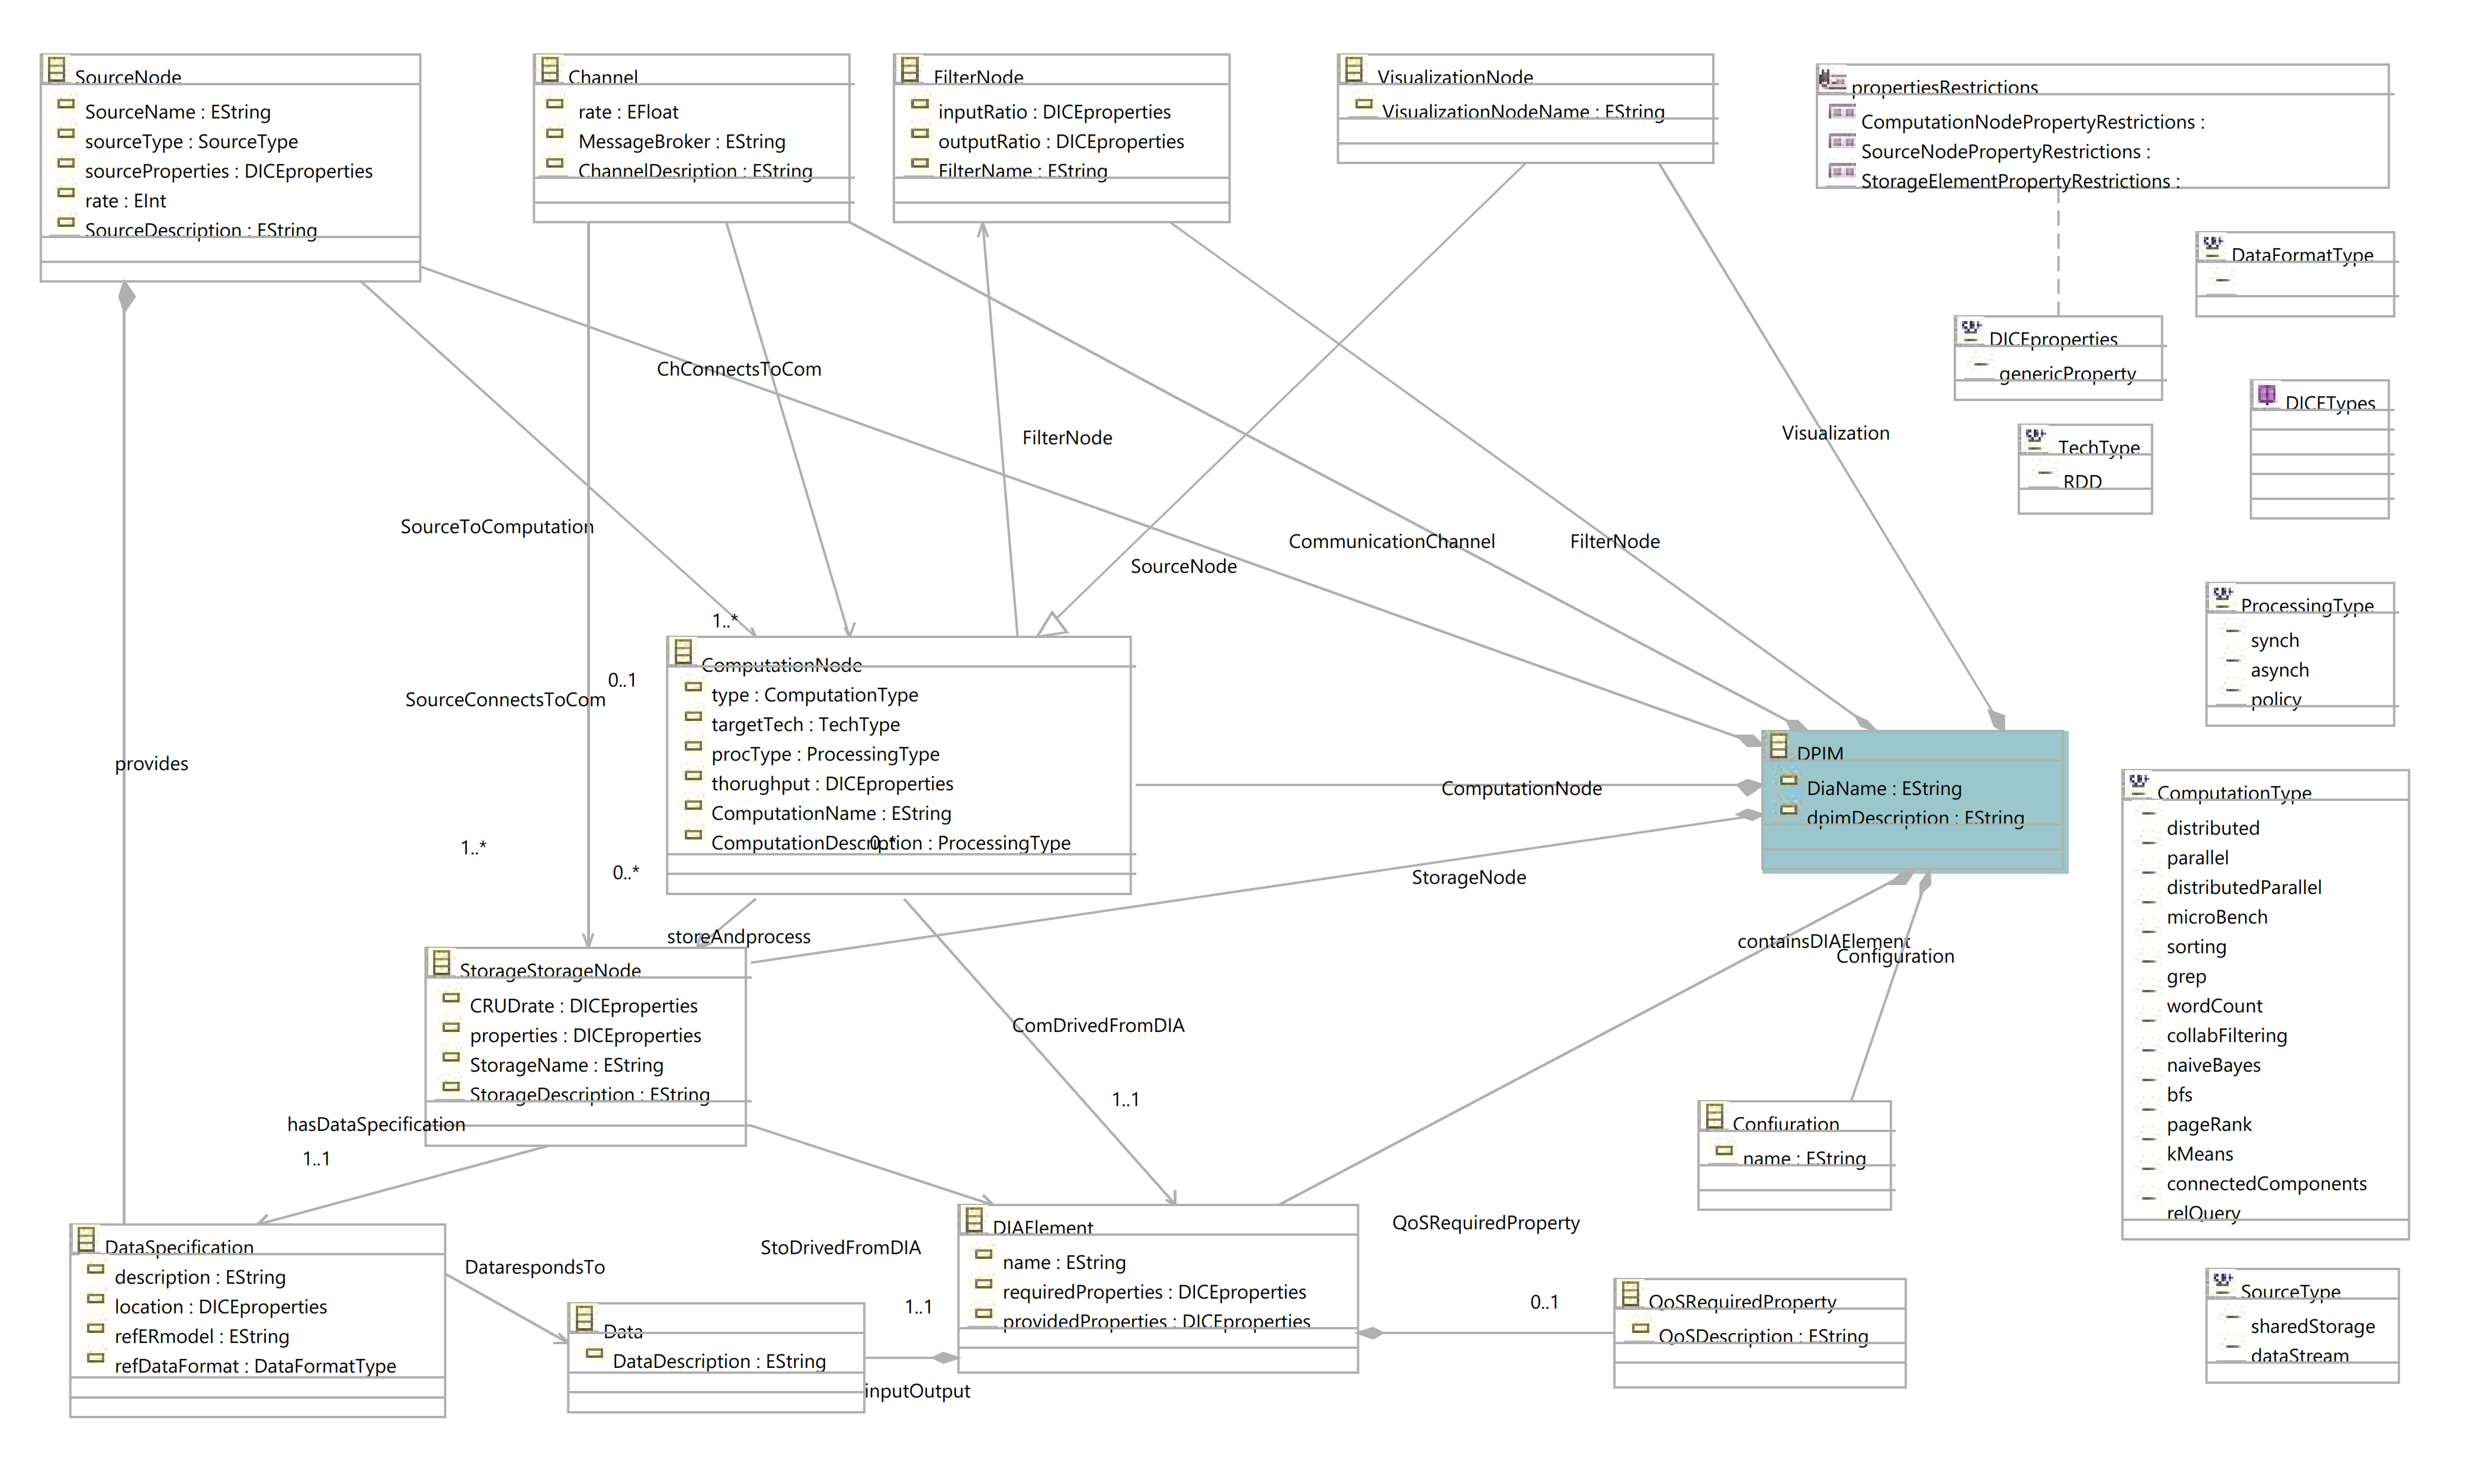
\includegraphics[width=\textwidth]{Images/11.png}
\caption{\label{fig:metamodel}DICE DPIM metamodel.}
\end{sidewaysfigure}

\begin{figure}
\centering
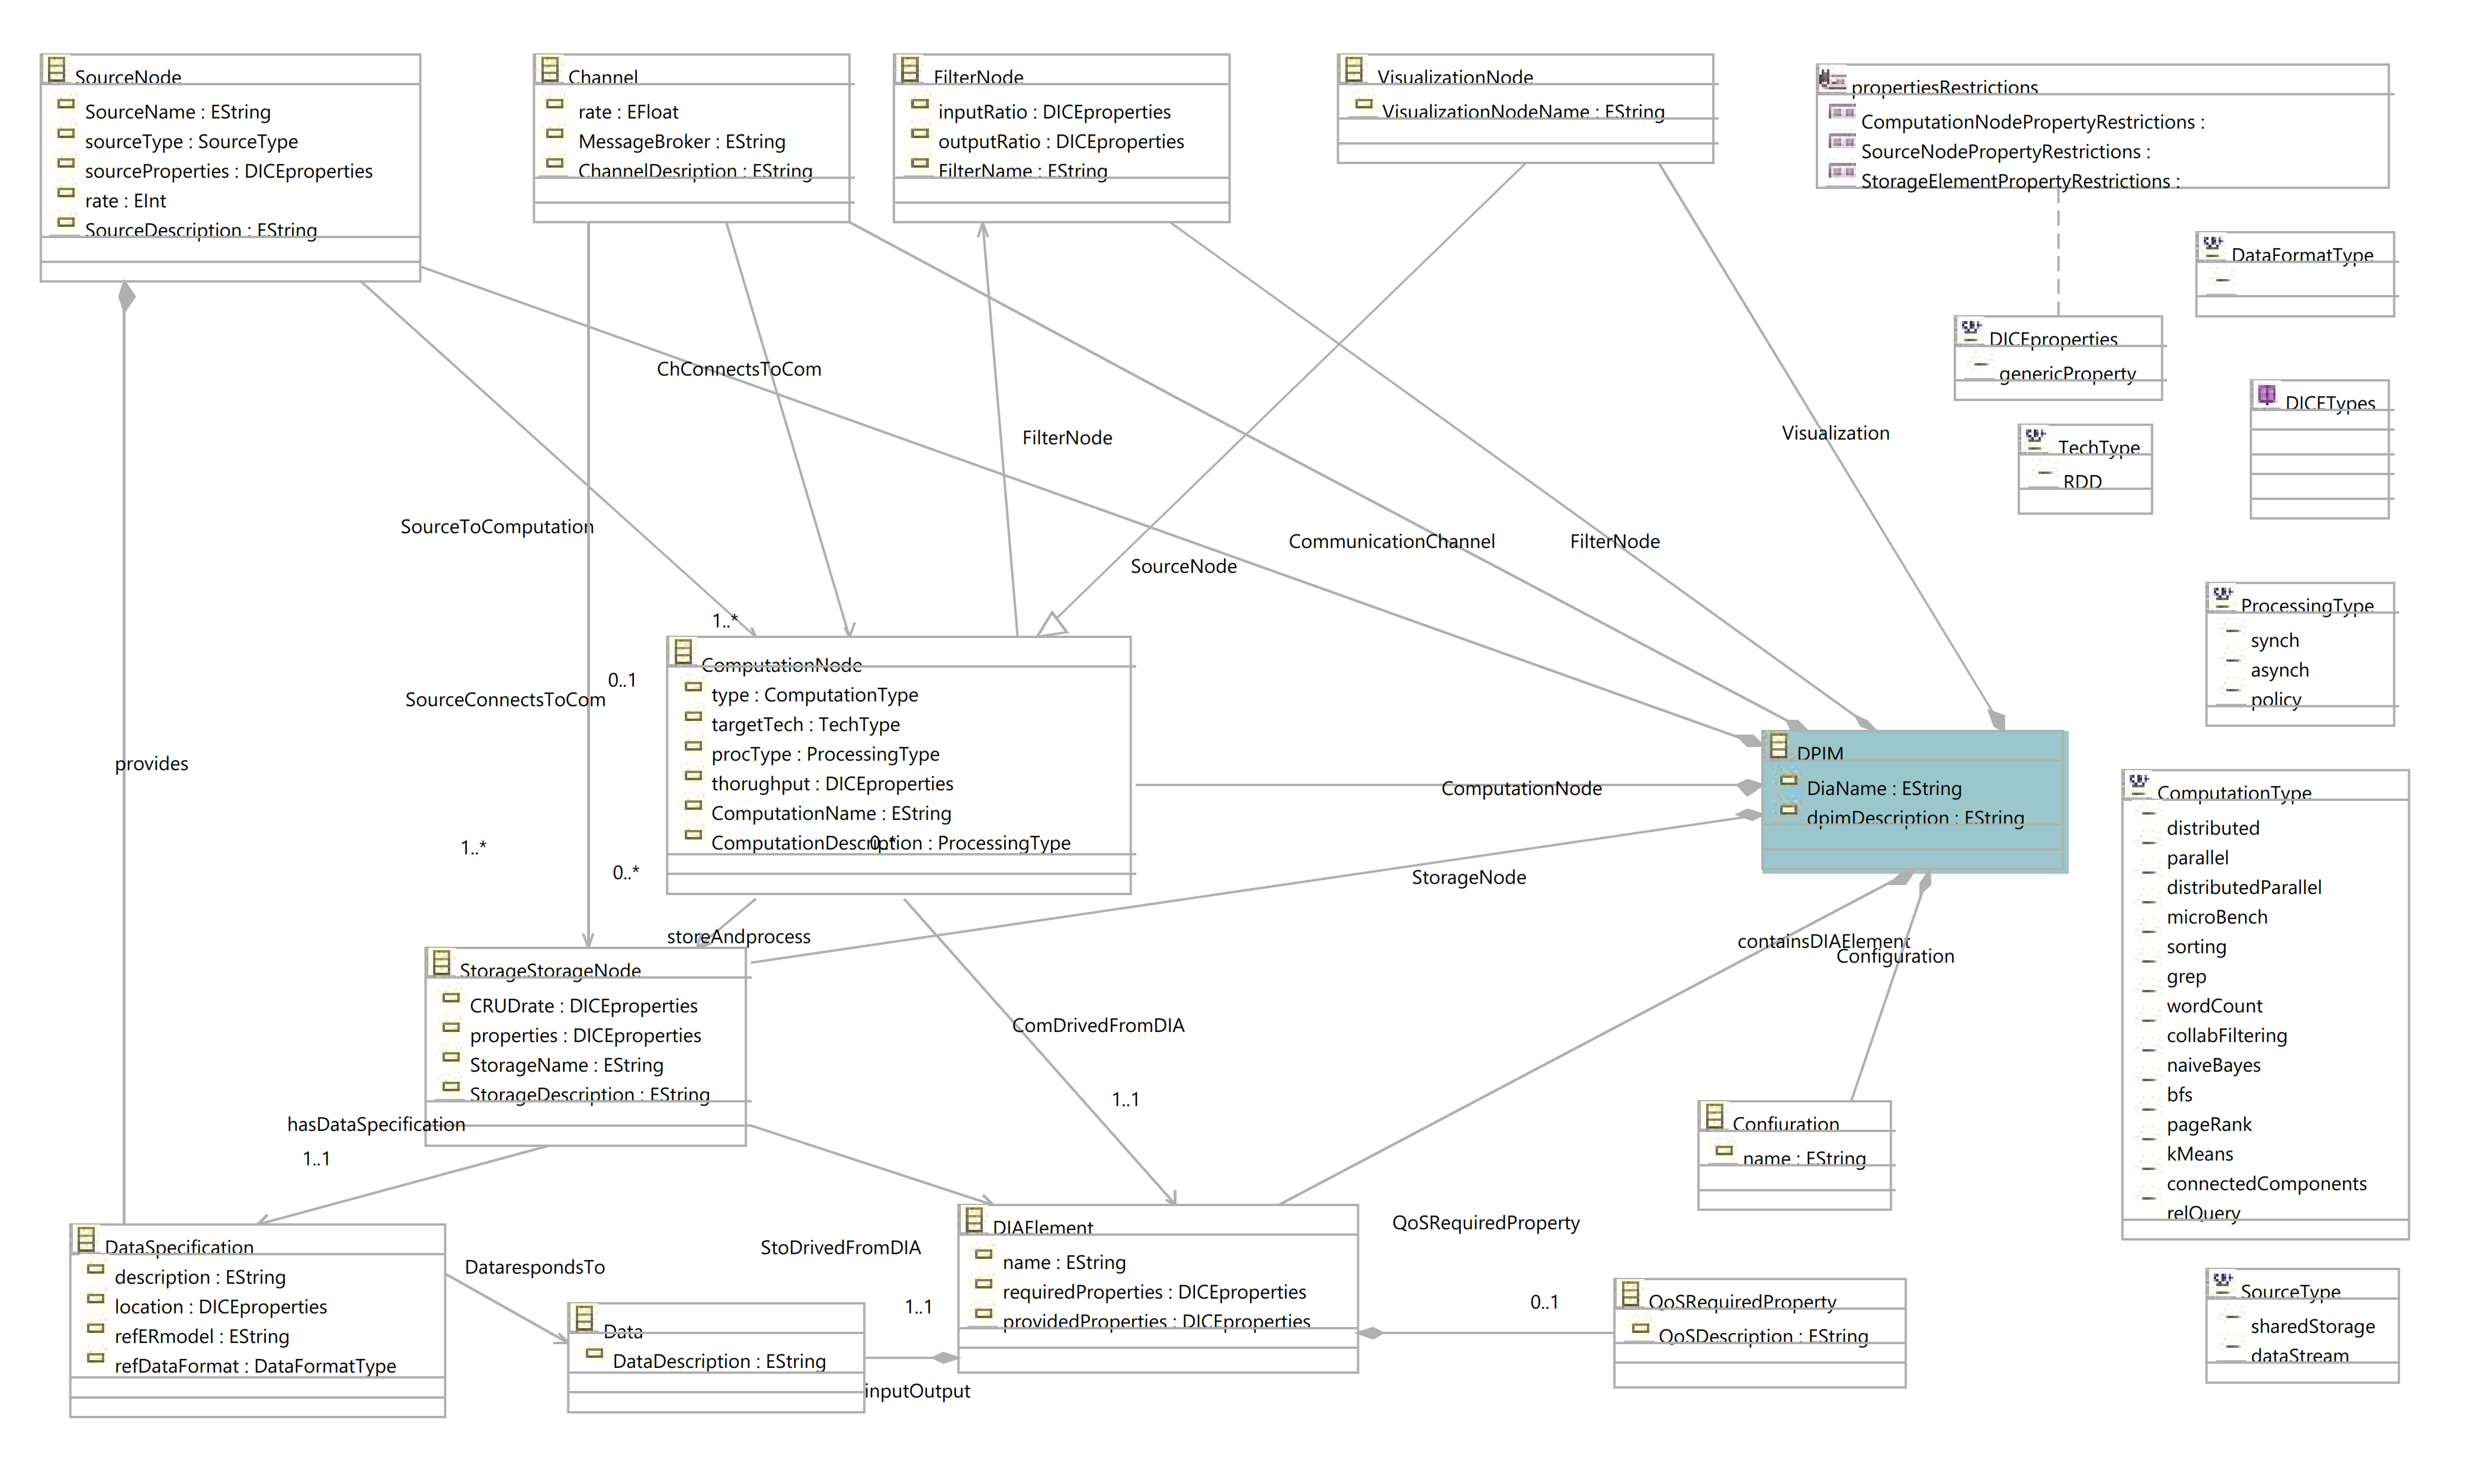
\includegraphics[width=\textwidth]{Images/11.png}
\caption{\label{fig:metamodel2}DICE DPIM metamodel in portrait form.}
\end{figure}

Here is the command to refer to another element (section, figure, table, ...) in the document: \emph{As discussed in Section~\ref{sect:overview} and as shown in Figure~\ref{fig:metamodel}, ...}. Here is how to introduce a bibliographic citation~\cite{DAM}. Bibliographic references should be included in a \texttt{.bib} file. 

Table generation is a bit complicated in Latex. You will soon become proficient, but to start you can rely on tools or external services. See for instance this \href{https://www.tablesgenerator.com}{https://www.tablesgenerator.com}. 


%------------------------------------------------------------------------------------------------------------------------------------------------
\clearpage
{\color{Blue}{\section{Specific Requirements}}}
\label{sect:requirements}
To further clarify and reason the implementation components proposed in the \textbf{\hyperref[fig:componentdiagram1]{main component diagram}} this chapter connects them with the goals and requirements, specified in the RASD document. Each goal \textbf{[Gn]} will be presented, and connected with the mapped requirements \textbf{[Rn]} and responsible design counterparts.\newline


\begin{table}[H]
\begin{flushleft}
\begin{tabular}{|l|l|}
\hline
R1&The user must be able to select a specific store in which they want \\ & to do the shopping.\\
\hline
R2&The user must be able to request a number and a ticket.\\
\hline
R3&The user must be able to receive a number and a ticket. \\
\hline
R4&The user must be able to physically retrieve a ticket from the printer \\   &  containing a number and a QR code.\\
\hline
R5&A new ticket must be printed whenever a user physically retrieves the old one.\\
\hline
R6&The store manager must be able to scan a QR code.\\
\hline
R7&The store manager must be informed by the application if a user tries to enter the \\ & store out of order.\\
\hline
R8&The store manager must be informed when the capacity of the store is full.\\
\hline
R9&The store manager must be able to alert the system whenever a customer \\ & exits the store.\\
\hline
R10&The store manager must be provided with the login credentials upon \\ & request to the system administrator.\\
\hline
R11&Allow the user to receive a precise estimation of waiting time when \\ &  retrieving a number.\\
\hline
R12&The system must calculate an estimation of the waiting time based on data.\\
\hline
R13&The system must be able to update its estimated waiting time in real time.\\
\hline
R14&The system must be able to send an update to the user in specific \\ & intervals regarding estimated waiting time until it's their turn.\\
\hline
R15&The user must be able to request to see all the available timeslots  in that \\ & specific store.\\
\hline
R16&The system must be able to provide the user with the list of all available timeslots \\ & upon the request.\\
\hline
R17&The user must be able to select a specific timeslot.\\
\hline
R18&The user must be able to receive a confirmation of his timeslot reservation, along \\ & with a number and a ticket.\\
\hline
R19&Allow the user to be at most five minutes late for his reservation before cancelling \\ &  his ticket.\\
\hline
R20&The user must be able to specify expected duration of his visit to the store.\\
\hline
\end{tabular}
\end{flushleft}
\caption{\textbf{Requirements table}}
\label{tab:reqtable}
\end{table}

\newpage
\begin{table}
\begin{flushleft}
\begin{tabular}{|l|l|}
\hline
\cellcolor[HTML]{EC8D78}& \cellcolor[HTML]{F4D5CE}Allow the user to retrieve a number through the application.\\
\cline{2-2}
\cellcolor[HTML]{EC8D78}& \cellcolor[HTML]{F4D5CE}Requirements: R1, R2, R3\\
\cline{2-2}
\cellcolor[HTML]{EC8D78}&Components:\\

\cellcolor[HTML]{EC8D78}G1.1&\quad\quad AndroidApp/IPhoneApp\\

\cellcolor[HTML]{EC8D78}&\quad\quad	Director \\

\cellcolor[HTML]{EC8D78}&\quad\quad	StoreSelectionManager \\

\cellcolor[HTML]{EC8D78}&\quad\quad	RequestManager \\

\cellcolor[HTML]{EC8D78}&\quad\quad\quad\quad	TicketService \\

\cellcolor[HTML]{EC8D78}&\quad\quad\quad\quad	QueueService \\

\cellcolor[HTML]{EC8D78}&\quad\quad\quad\quad	ScheduleService\\ 

\cellcolor[HTML]{EC8D78}&\quad\quad	DBService and DB \\
\hline
\end{tabular}
\end{flushleft}
\caption{\textbf{Components table - Goal 1.1}}
\label{tab:comp1}
\end{table}


\begin{table}
\begin{flushleft}
\begin{tabular}{|l|l|}
\hline
\cellcolor[HTML]{EC8D78}& \cellcolor[HTML]{F4D5CE}Allow the user to retrieve a number physically from the printer.\\
\cline{2-2}
\cellcolor[HTML]{EC8D78}& \cellcolor[HTML]{F4D5CE}Requirements: R4, R5 \\
\cline{2-2}
\cellcolor[HTML]{EC8D78}&Components:\\

\cellcolor[HTML]{EC8D78}G1.2&\quad\quad	Director \\

\cellcolor[HTML]{EC8D78}&\quad\quad	StoreSelectionManager \\

\cellcolor[HTML]{EC8D78}&\quad\quad	RequestManager \\

\cellcolor[HTML]{EC8D78}&\quad\quad\quad\quad	TicketService \\

\cellcolor[HTML]{EC8D78}&\quad\quad\quad\quad	QueueService \\

\cellcolor[HTML]{EC8D78}&\quad\quad\quad\quad	ScheduleService\\ 

\cellcolor[HTML]{EC8D78}&\quad\quad	DBService and DB \\
\hline
\end{tabular}
\end{flushleft}
\caption{\textbf{Components table - Goal 1.2}}
\label{tab:comp1}
\end{table}

\begin{table}
\begin{flushleft}
\begin{tabular}{|l|l|}
\hline
\cellcolor[HTML]{EC8D78}& \cellcolor[HTML]{F4D5CE}Allow the store manager to control the entrance of customers via QR code scanning.\\
\cline{2-2}
\cellcolor[HTML]{EC8D78}& \cellcolor[HTML]{F4D5CE}Requirements: R6, R7, R8, R9, R10\\
\cline{2-2}
\cellcolor[HTML]{EC8D78}&Components:\\

\cellcolor[HTML]{EC8D78}G2&\quad\quad AndroidApp/IPhoneApp\\

\cellcolor[HTML]{EC8D78}&\quad\quad	Director \\

\cellcolor[HTML]{EC8D78}&\quad\quad	LoginManager \\

\cellcolor[HTML]{EC8D78}&\quad\quad	StoreSelectionManager \\

\cellcolor[HTML]{EC8D78}&\quad\quad	StoreManager \\

\cellcolor[HTML]{EC8D78}&\quad\quad\quad\quad EnterService \\

\cellcolor[HTML]{EC8D78}&\quad\quad\quad\quad ExitService \\

\cellcolor[HTML]{EC8D78}&\quad\quad	RequestManager \\

\cellcolor[HTML]{EC8D78}&\quad\quad	DBService and DB \\
\hline
\end{tabular}
\end{flushleft}
\caption{\textbf{Components table - Goal 2}}
\label{tab:comp1}
\end{table}


\newpage

\begin{table}
\begin{flushleft}
\begin{tabular}{|l|l|}
\hline
\cellcolor[HTML]{EC8D78}& \cellcolor[HTML]{F4D5CE}Allow the user to receive precise calculations of the waiting time.\\
\cline{2-2}
\cellcolor[HTML]{EC8D78}& \cellcolor[HTML]{F4D5CE}Requirements: R11, R12\\
\cline{2-2}
\cellcolor[HTML]{EC8D78}&Components:\\

\cellcolor[HTML]{EC8D78}G3&\quad\quad AndroidApp/IPhoneApp\\

\cellcolor[HTML]{EC8D78}&\quad\quad	Director \\

\cellcolor[HTML]{EC8D78}&\quad\quad	RequestManager \\

\cellcolor[HTML]{EC8D78}&\quad\quad\quad\quad	DistanceService \\

\cellcolor[HTML]{EC8D78}&\quad\quad	GoogleMapsService\\ 

\cellcolor[HTML]{EC8D78}&\quad\quad	DBService and DB \\
\hline
\end{tabular}
\end{flushleft}
\caption{\textbf{Components table - Goal 3}}
\label{tab:comp1}
\end{table}



\begin{table}
\begin{flushleft}
\begin{tabular}{|l|l|}
\hline
\cellcolor[HTML]{EC8D78}& \cellcolor[HTML]{F4D5CE}Allow the user to be updated on the store waiting time situation.\\
\cline{2-2}
\cellcolor[HTML]{EC8D78}& \cellcolor[HTML]{F4D5CE}Requirements: R13, R14\\
\cline{2-2}
\cellcolor[HTML]{EC8D78}&Components:\\

\cellcolor[HTML]{EC8D78}G4&\quad\quad AndroidApp/IPhoneApp\\

\cellcolor[HTML]{EC8D78}&\quad\quad	Director \\

\cellcolor[HTML]{EC8D78}&\quad\quad	RequestManager \\

\cellcolor[HTML]{EC8D78}&\quad\quad	GoogleMapsService \\

\cellcolor[HTML]{EC8D78}&\quad\quad	DBService and DB \\
\hline
\end{tabular}
\end{flushleft}
\caption{\textbf{Components table - Goal 4}}
\label{tab:comp1}
\end{table}




\begin{table}
\begin{flushleft}
\begin{tabular}{|l|l|}
\hline
\cellcolor[HTML]{EC8D78}& \cellcolor[HTML]{F4D5CE}Allow the user to "book a visit" to the store.\\
\cline{2-2}
\cellcolor[HTML]{EC8D78}& \cellcolor[HTML]{F4D5CE}Requirements: R15, R16, R17, R18, R19, R20\\
\cline{2-2}
\cellcolor[HTML]{EC8D78}&Components:\\

\cellcolor[HTML]{EC8D78}G5&\quad\quad AndroidApp/IPhoneApp\\

\cellcolor[HTML]{EC8D78}&\quad\quad	Director \\

\cellcolor[HTML]{EC8D78}&\quad\quad	StoreSelectionManager \\

\cellcolor[HTML]{EC8D78}&\quad\quad	RequestManager \\

\cellcolor[HTML]{EC8D78}&\quad\quad\quad\quad	BookAVisitService \\

\cellcolor[HTML]{EC8D78}&\quad\quad\quad\quad	TicketService \\

\cellcolor[HTML]{EC8D78}&\quad\quad\quad\quad	QueueService\\ 

\cellcolor[HTML]{EC8D78}&\quad\quad\quad\quad	ScheduleService\\ 

\cellcolor[HTML]{EC8D78}&\quad\quad	DBService and DB \\
\hline
\end{tabular}
\end{flushleft}
\caption{\textbf{Components table - Goal 5}}
\label{tab:comp1}
\end{table}



%------------------------------------------------------------------------------------------------------------------------------------------------
\clearpage
{\color{Blue}{\section{Formal Analysis Using Alloy}}}
\label{sect:alloy}
\begin{lstlisting}[language=alloy]
open util/integer

abstract sig TixState{}

one sig WAITING extends TixState{}
one sig INSTORE extends TixState{}
one sig EXPIRED extends TixState{}

abstract sig Location{}
sig GPSCoordinates extends Location {
	store: some Store

	// GPSCoordinates have been simplified for clearer view

	//latitude: one Int,
	//longitude: one Int
	}	
	/*{
		latitude < 90 and latitude > -90
		longitude < 180 and longitude > -180
	}*/

// Simplified version of address only includes GPSCoordinates
/*
sig Address extends Location {
	country: one Country,
	city: one City,
	street: one Street,
	number: one Int
	}

*/

  // Working time has been simplified for clearer view
sig WorkingTime{
	store: some Store
	}


	// One buyer has one ticket and optional GPS coordinates
sig Buyer{
	ticket: one Ticket,
	locGPS: lone GPSCoordinates,
}

sig QRCode{}

sig Store{
	allTickets: set Ticket,
	maxCustomers: one Int,
	storeId: one Int,
	timeOfWork: one WorkingTime,
	locGPS: one GPSCoordinates,
}{
	maxCustomers > 0 and storeId > 0
}


	// A tickets has a number, a parent store, a ticket state, and a QR code
	// Ticket state can be WAITING if the ticket is still in queue,
	// INSTORE if the buyer entered the store, and EXPIRED, if the 
	// ticket has expired
sig Ticket{
	tixNum: one Int,
	parentStore: one Store,
	tixState: one TixState,
	qr: one QRCode
}{
	tixNum > 0 and tixNum <= parentStore.maxCustomers
}

    // There must be less tickets than the number of maximum customers
fact {
	(all s:Store | #s.allTickets < s.maxCustomers)
}

    // No two tickets with the same number can exist in the same store
fact {
	all disj t1,t2:Ticket | (t1.tixNum != t2.tixNum and t1.parentStore = t2.parentStore ) 
}

	// Every ticket must have only one owner (buyer)
fact{
	all disj b1,b2:Buyer | (b1.ticket != b2.ticket)
}

fact {
	all disj s1,s2:Store | s1.storeId != s2.storeId
}

	// Every ticket has to belong to only one store
fact {
	(all s:Store | all t:s.allTickets | t.parentStore.storeId = s.storeId)
}

fact {
	(all s:Store | all w:WorkingTime | #s >= #w) 
}


pred show{
	(some s:Store | #s.allTickets > 1 )
}

run show 
\end{lstlisting}

\newpage

\begin{figure}[!htb]
\centering
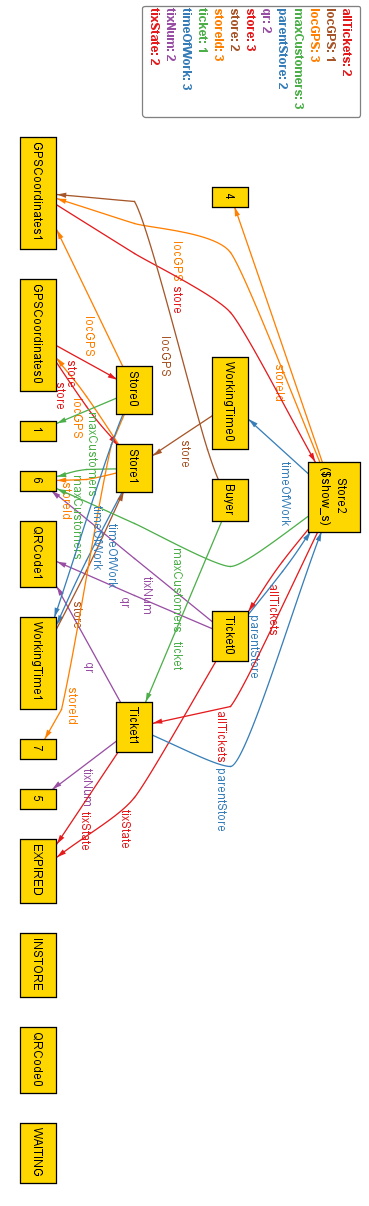
\includegraphics[width=0.38\textwidth]{Images/AlloyGraph1V}
\caption{\label{fig:alloy1}\textbf{Alloy graph 1}}
\end{figure}

\newpage

\begin{figure}[!htb]
\centering
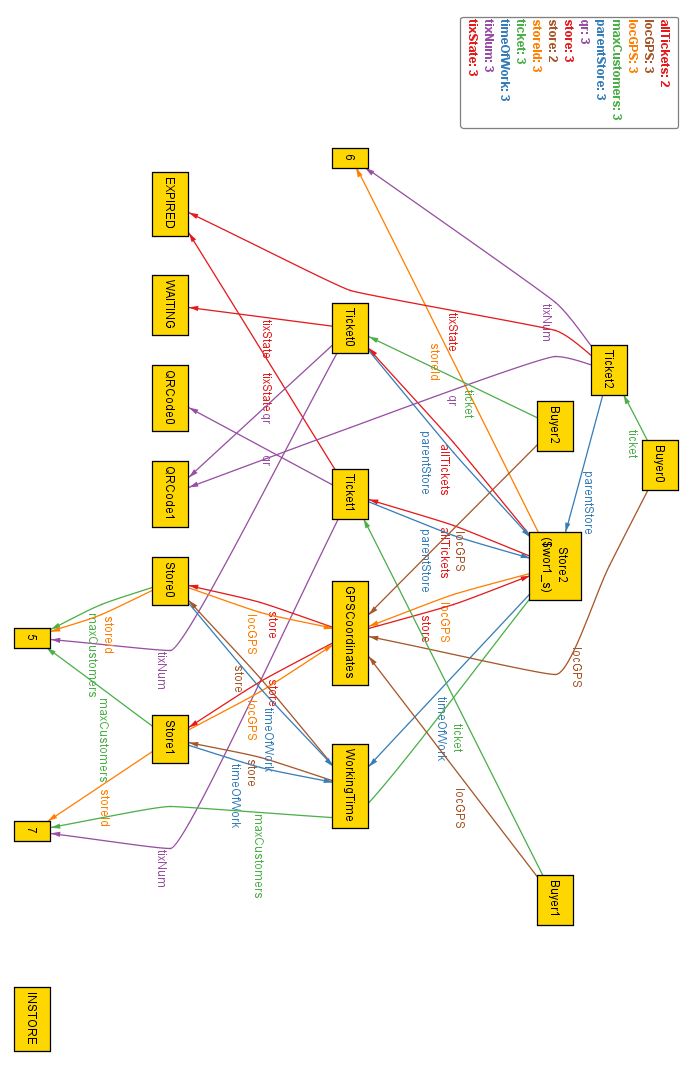
\includegraphics[width=0.8\textwidth]{Images/AlloyGraph2V}
\caption{\label{fig:alloy2}\textbf{Alloy graph 2}}
\end{figure}

%------------------------------------------------------------------------------------------------------------------------------------------------
\clearpage
{\color{Blue}{\section{Effort Spent}}}
\label{sect:effort}
\begin{table}[!htb]
\centering
\begin{tabular}{|
>{\columncolor[HTML]{EFEFEF}}l |l|}
\hline
\cellcolor[HTML]{C0C0C0}\textbf{Task Description}                                                   & \cellcolor[HTML]{C0C0C0}\textbf{Time spent{[}hours{]}} \\ \hline
\begin{tabular}[c]{@{}l@{}}Introduction:\\ \\ \end{tabular} &                                                   1 \\ \hline
\begin{tabular}[c]{@{}l@{}}Overall description:\\ Product perspective and functions, user characteristics, and constraints\end{tabular} &  5\\ \hline
\begin{tabular}[c]{@{}l@{}}Overall description:\\ Goals, Assumptions, and Dependencies\end{tabular} &                                                    2 \\ \hline
\begin{tabular}[c]{@{}l@{}}Specific requirements:\\ External interface Requirements\end{tabular}    &                                                       2 \\ \hline
\begin{tabular}[c]{@{}l@{}}Specific requirements:\\ Use Case diagrams\end{tabular}                  &                                                       5 \\ \hline
\begin{tabular}[c]{@{}l@{}}Formal analysis using Alloy:\\ \\ \end{tabular} &                                                       6 \\ \hline
\begin{tabular}[c]{@{}l@{}}LaTex document composition:\\ \\ \hline \end{tabular} &                                                        12\\ \hline
\begin{tabular}[c]{@{}l@{}}Total:\\ \\ \hline \end{tabular} &                                                        33\\ \hline
\end{tabular}
\caption{\textbf{Effort spent - Robert Medvedec}}
\label{tab:my-table}
\end{table}


\begin{table}[!htb]
\centering
\begin{tabular}{|
>{\columncolor[HTML]{EFEFEF}}l |l|}
\hline
\cellcolor[HTML]{C0C0C0}\textbf{Task Description}                                                   & \cellcolor[HTML]{C0C0C0}\textbf{Time spent{[}hours{]}} \\ \hline
\begin{tabular}[c]{@{}l@{}}Introduction:\\ \\ \end{tabular} &                                                        \\ \hline
\begin{tabular}[c]{@{}l@{}}Overall description:\\ Product perspective and functions, user characteristics, and constraints\end{tabular} &  \\ \hline
\begin{tabular}[c]{@{}l@{}}Overall description:\\ Goals, Assumptions, and Dependencies\end{tabular} &                                                        \\ \hline
\begin{tabular}[c]{@{}l@{}}Specific requirements:\\ External interface Requirements\end{tabular}    &                                                        \\ \hline
\begin{tabular}[c]{@{}l@{}}Specific requirements:\\ Use Case diagrams\end{tabular}                  &                                                        \\ \hline
\begin{tabular}[c]{@{}l@{}}Formal analysis using Alloy:\\ \\ \end{tabular} &                                                        \\ \hline
\begin{tabular}[c]{@{}l@{}}LaTex document composition:\\ \\ \end{tabular} &                                                        \\ \hline
\begin{tabular}[c]{@{}l@{}}Total:\\ \\ \hline \end{tabular} &                                                        \\ \hline
\end{tabular}
\caption{\textbf{Effort spent - Toma Sikora}}
\label{tab:my-table}
\end{table}


%------------------------------------------------------------------------------------------------------------------------------------------------
\clearpage
\addcontentsline{toc}{section}{References}
\bibliographystyle{plain}
\bibliography{main}
%------------------------------------------------------------------------------------------------------------------------------------------------




\end{document}
